\section{Understanding Rollup}
One of the predominant time savers in GUFI is the rollup feature which functions like so: \\
\begin{itemize}
  \item contents of the child's summary table are copied up with name column to include the parent directory
  \item pentries view/table is dropped and a pentries table is created with the data inside the pentries view/table
  \item copy child's pentries view into parent (regardless if view or table)
  \item ALL children must be able to rollup
\end{itemize}


\begin{figure} [h]
\centering
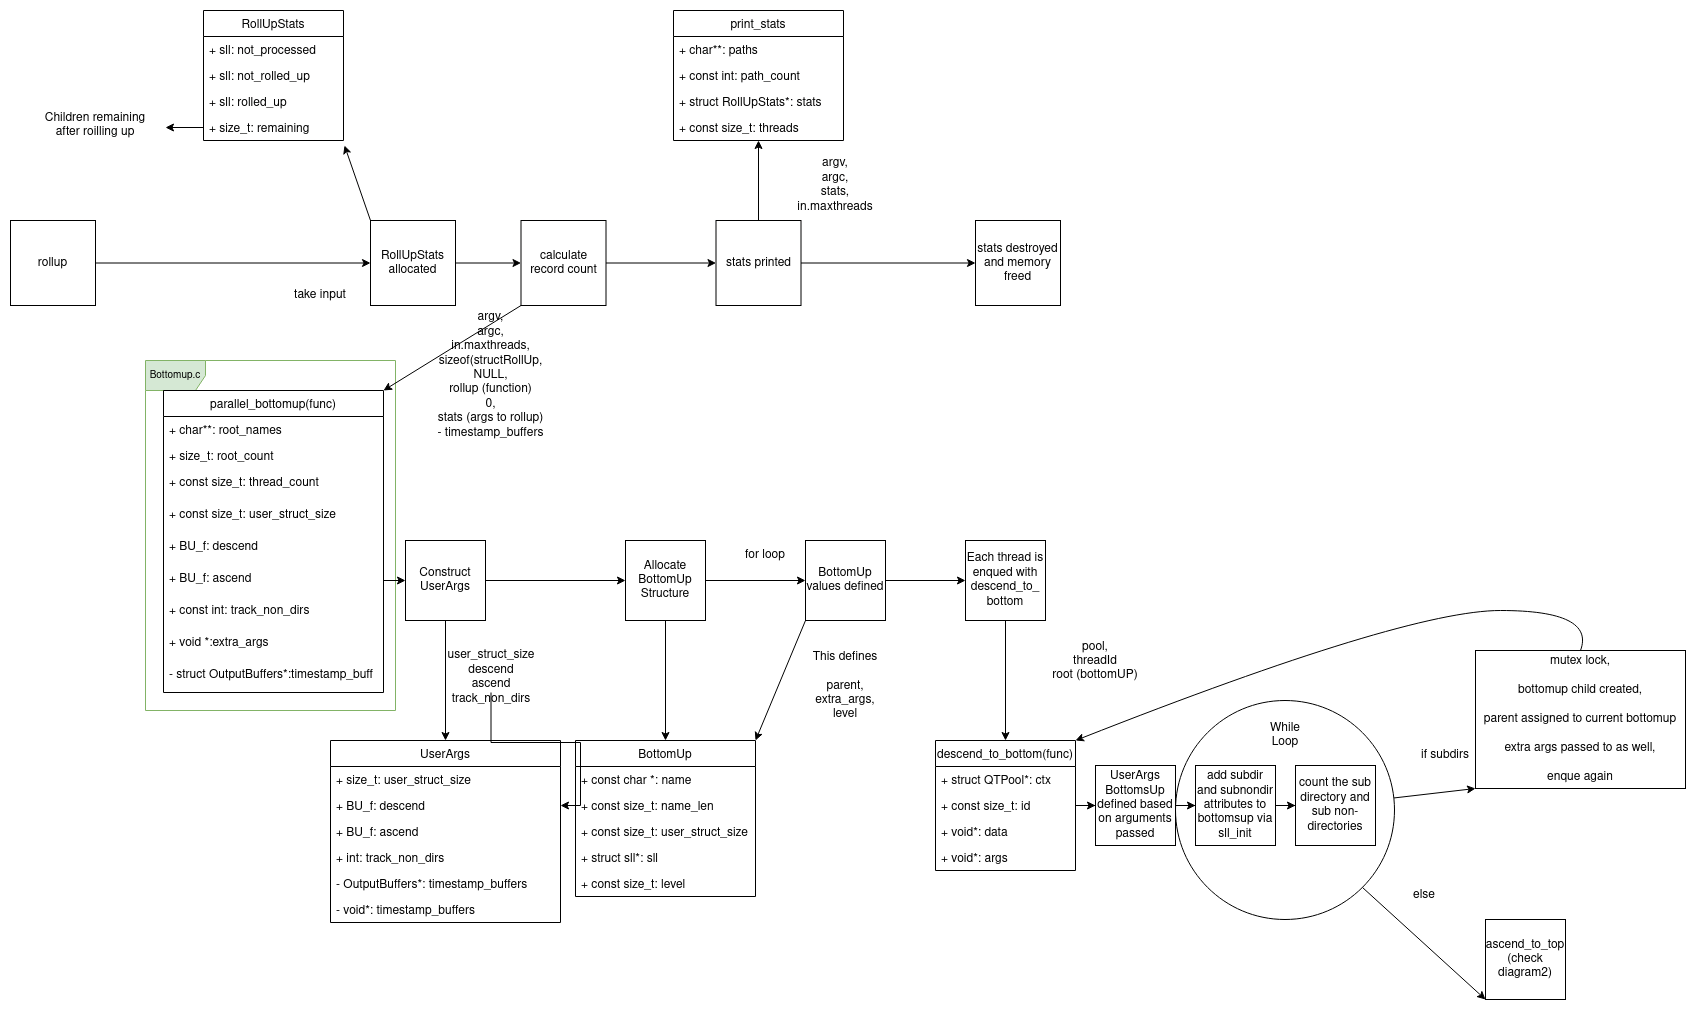
\includegraphics[width=1.2\textwidth]{images/rollup.png}
\caption{\label{fig:rollup}Rollup Workflow}
\end{figure}


\begin{figure} [h]
\centering
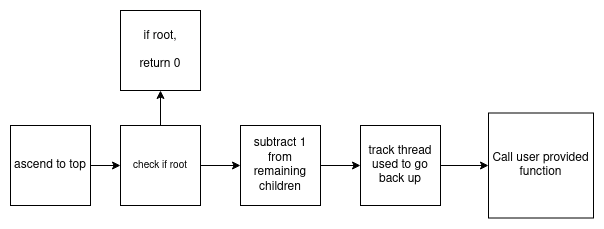
\includegraphics[width=0.8\textwidth]{images/ascending.png}
\caption{\label{fig:gufi_query} Ascending Workflow}
\end{figure}

\clearpage